\chapter{序論}
%%\cite{thrun2005probabilistic}
\section{はじめに}
 今日の日本は少子高齢化の影響による労働人口の減少に直面しており, その中でも運送業界やタクシー業界などでは深刻なドライバーの高齢化と働き手となる若者の不足に直面している. そのような状況下において自動運転技術の実用化に対する期待は非常に大きい. その中で自動運転の核となる技術である自己位置推定は古くから研究が進められてきた.自己位置推定には図\ref{fig:3D-PointCloud}のような点群データが得られるLiDAR(図\ref{fig:HDL-64E})やカメラ, GPSなどの機器が使用される. 近年ではカメラによる自己位置推定, 通称ビジュアルローカリゼーションを季節や時間などによる景色の光学的な変化に対して頑強にしようとする研究が盛んに行われている\cite{semantic_segmentation_in_snow}\cite{stenborg_2020}. 
\begin{figure}[htpb]
\begin{center}
\begin{tabular}{cc}
\begin{minipage}[t]{1.0\hsize}
\begin{center}
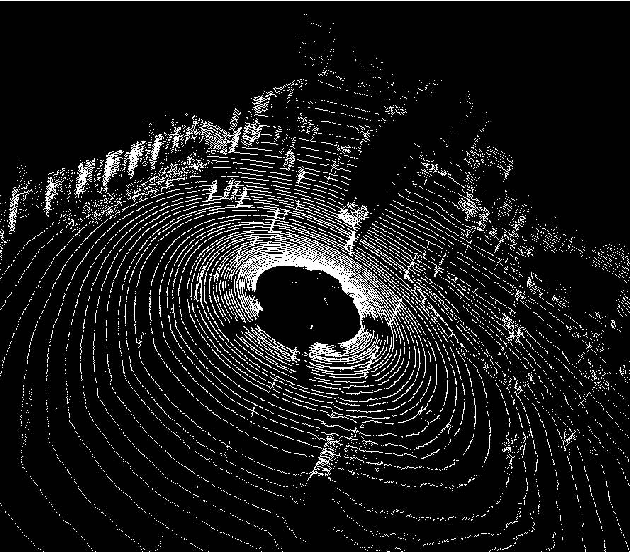
\includegraphics[width=5cm]{./picture/KITTI_pointcloud.png}
\caption{LiDARから得られた三次元点群}
\label{fig:3D-PointCloud}
\end{center}
\end{minipage} \\ \\
\begin{minipage}[t]{1.0\hsize}
\begin{center}
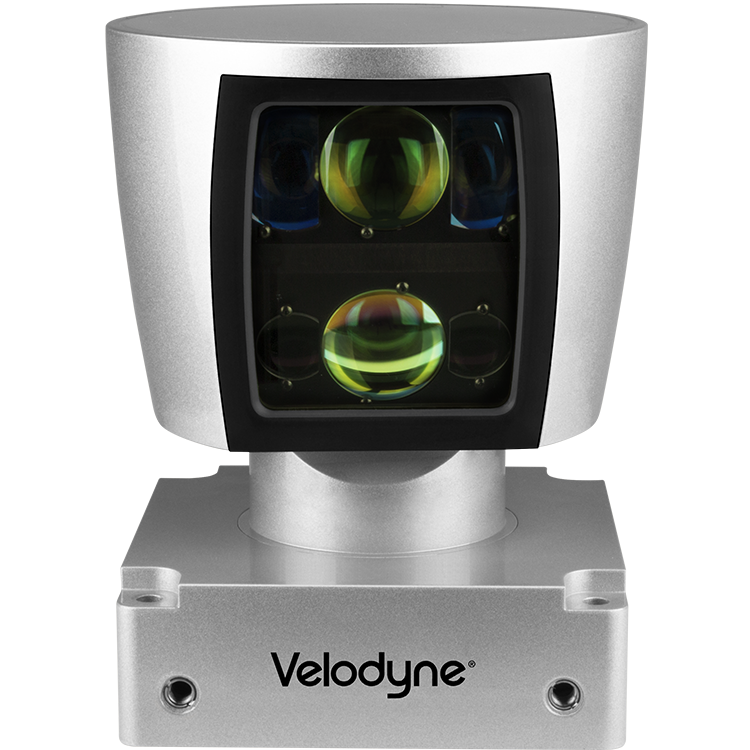
\includegraphics[width=5cm]{./picture/HDL64E.png}
\caption{Velodyne HDL-64E}
\label{fig:HDL-64E}
\end{center}
\end{minipage}
\end{tabular}
\end{center}
\end{figure}

\newpage
 
 \section{研究背景}
 ロボティクスにおいて自己位置推定は重要課題の一つである\cite{thrun2005probabilistic}. 自己位置推定の主なタスクはすでに構築された地図とロボットに搭載されたセンサからのデータを利用して確率統計学のアプローチから最もロボットが存在する確率の高い場所を算出することである。このときに使用されるセンサにはLiDARやカメラ, GPSなどが一般的でありその中でもカメラは比較的小型で安価であることから幅広い分野のロボットで使われている, ロボット掃除機の代表格でもあるiRobot社製のRoombaでもカメラによるビジュアルローカリゼーションを行っている\cite{Roomba_vSLAM}. \par ビジュアルローカリゼーションでは地図生成の際に抽出したエッジ\cite{Wuhan_Edge_Locali}やSIFTなどを始めとする特徴記述子等を三次元空間地図におけるランドマークとして配置し, ロボット搭載のカメラ画像から抽出した特徴量と比較することでロボット自身の位置を推定している\cite{vslam_survey}. 自動運転などを始めとするロボティクスの分野においてカメラから得られる情報は非常に使い勝手がよく, 先述のビジュアルローカリゼーションだけでなく人や車の検出など幅広く使われている\cite{DeepLab}. \par しかし, ビジュアルローカリゼーションにおいて頻繁に使用される特徴記述子には実用上で大きな問題が存在する. それは特徴記述子の抽出はコントラスト変化に対してはロバストであるものの, 昼と夜などの時間による景色の変化や季節変化による木や植物の色や日光のあたり方などの環境の変化には対応しきれないという点である\cite{Image_Recog_Kodansha}. さらにPedersonらの研究\cite{FeatureDescriptor}では一般的に使用されているSIFTやSURFなどの特徴記述子は光の状態に関して非常に敏感な反応を示すことが書かれている. 
これは特徴記述子の抽出が環境変化に対してロバストな設計ができたとしても, 地図とのマッチングの際に毎回同じ値で特徴子の抽出はできないため, 地図上の特徴点と比較するビジュアルローカリゼーションでは正確な尤度算出をする上で妨げになることを示唆している. したがってビジュアルローカリゼーションにおいて現在求められているものは季節や時間による環境変化に対してロバストなビジュアルローカリゼーションを実現すること, およびそれをより高い精度にすることである. \par この問題に対して, \ref{sec:related_work}節で述べる手法は環境変化に対して頑強な自己位置推定を実現した. しかし, その手法は複数の実用上の問題が存在する. 本研究ではそれらの問題を解決し実用的な自己位置推定手法を提案することを目的とする.
 
\begin{figure}[htbp]
\begin{center}
\begin{tabular}{c}
\begin{minipage}{0.7\hsize}
\begin{center}
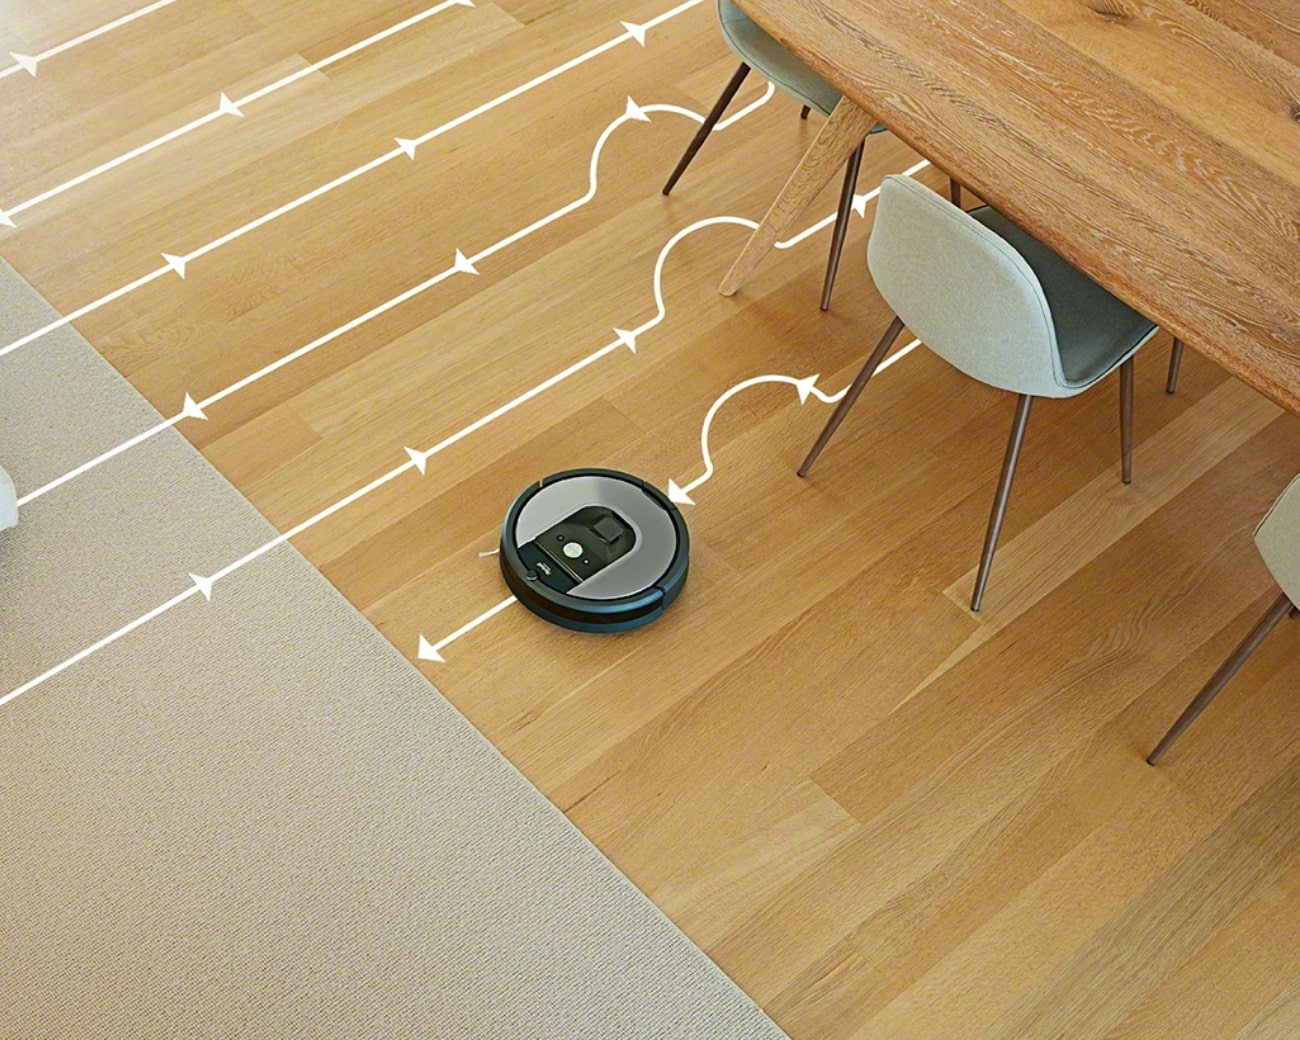
\includegraphics[width=10cm]{./picture/img-roomba.jpg}
\caption{iRobot社製 Roomba Series900}
\label{fig:Roomba}
\end{center}
\end{minipage}
\end{tabular}
\end{center}
\end{figure}

 \section{関連研究}\label{sec:related_work}
 先述の問題点に対して北海道大学の研究グループ\cite{semantic_segmentation_in_snow}とStenborgら\cite{semantic_point_localization}\cite{Toft_2018_ECCV}\cite{SattlerMTSPPO17}はそれぞれセマンティックセグメンテーションを地図生成とビジュアルローカリゼーションの両方で利用することで環境変化に対するロバスト性を実現しようとした. 機械学習を利用すれば季節の変化によって色や光の当たり方が変化したとしても学習時に同じ正解ラベルを与えることで図\ref{fig:ICNet}のようにセグメンテーションをする際には正しいクラスの出力結果が得られる. この特性を利用してStenborgらは図\ref{fig:SemanticPointLocalizationMap}のようにクラスごとに色分けされた三次元点群地図を生成, その地図の点とセグメンテーションしたカメラ画像をピクセル単位で比較することでビジュアルローカリゼーションを行った\cite{semantic_point_localization}. また, 地図にセマンティックな情報をもたせることで自己位置推定において地図上の木や建物などの物体が一種のランドマークとなる. これによってこれによって従来手法で用いられてきたQRコード\cite{QR_code_localization}や磁気マーカ\cite{jiki_marker_localization}などランドマークとなる人工物を設置する必要がないといったメリットが生まれる. \par この手法によって季節による特徴量抽出の変化の問題はある程度解決したが
2つの大きな問題が残った, 2つとも点群地図を使用することによるものである. 1つ目の問題点は点群地図はスパースな点で構成されているという問題であり, マッチングをする際には建物の裏側を構成する点群が図\ref{fig:Point_Cloud_Map}のように視界に入ってくるため住宅街など入り組んだ環境下ではピクセル単位で一致度を測定する時に尤度算出の妨げになる.2つ目はピクセル単位で点群地図と一致度を図る際に起こる問題点である. セグメンテーションされたカメラ画像と三次元のラベル付き点群地図をピクセル単位で比較する際, 点群地図だと少ない数の点でマッチングをする必要がある. これによって一つの点が持つ情報の重要度は相対的に上がり外乱などによるセグメンテーションの誤分類に脆弱になる. \par セマンティックな情報を地図生成と自己位置推定の両方に取り入れた研究はあまり多くなく, これらの問題に対して解決を図った研究は現時点で行われていない.
 
\begin{figure}[htbp]
\begin{tabular}{cc}
\begin{minipage}[t]{1.0\hsize}
\begin{center}
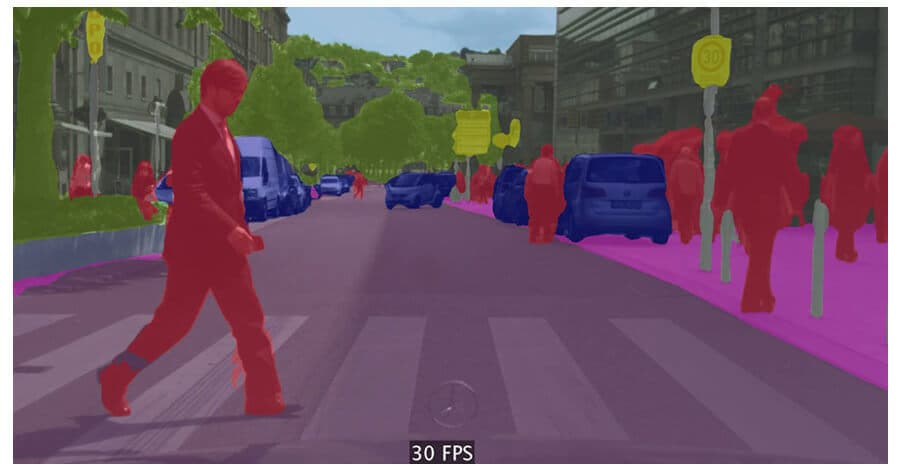
\includegraphics[width=14cm]{./picture/semseg.jpg}
\caption{セマンティックセグメンテーションの例}
\label{fig:ICNet}
\end{center}
\end{minipage} \\ \\
\begin{minipage}[t]{1.0\hsize}
\begin{center}
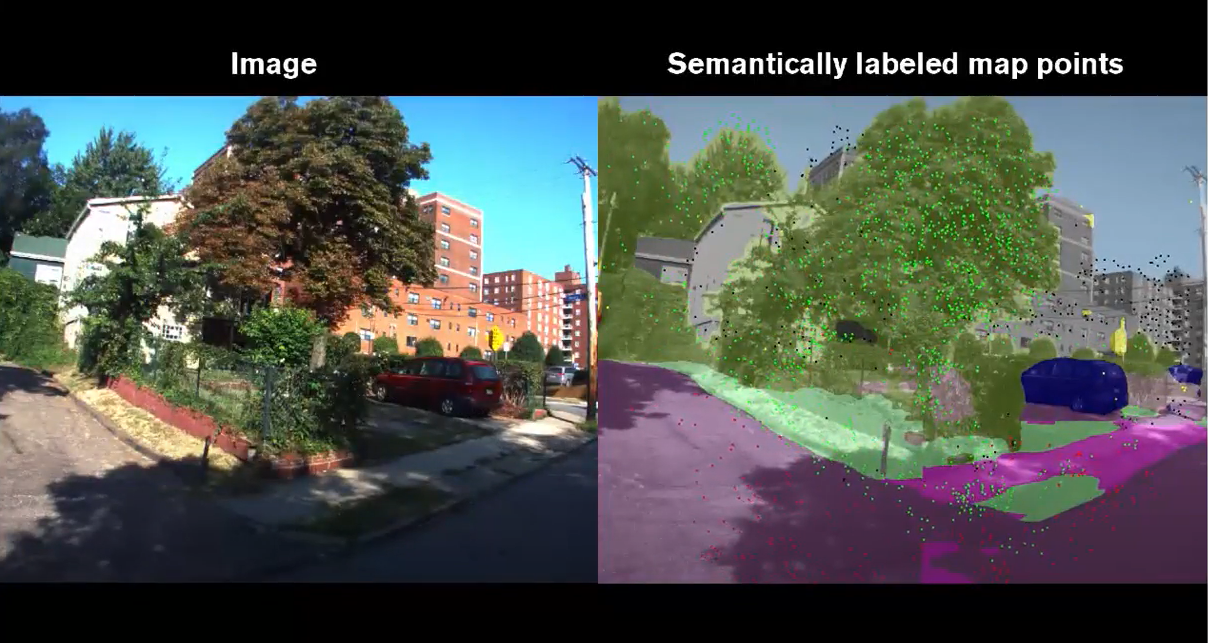
\includegraphics[width=14cm]{./picture/LongTermLocalization.png}
\caption{先行研究におけるカメラ画像(左), 及びラベル付けされた画像および点群地図(右)}
\label{fig:SemanticPointLocalizationMap}
\end{center}
\end{minipage} \\ \\
\begin{minipage}{1.0\hsize}
\begin{center}
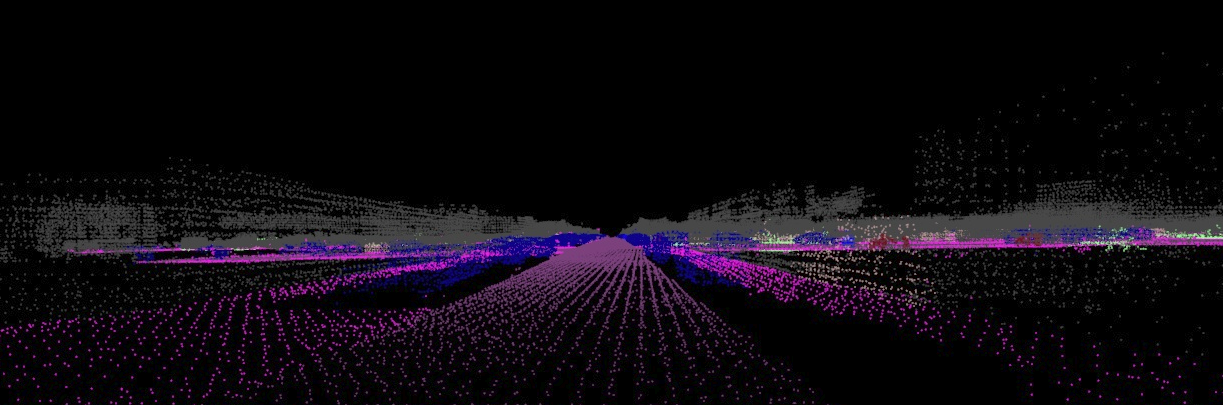
\includegraphics[width=14cm]{./picture/pc_map.png}
\caption{スパースな点群地図, 建物を構成する点群が手前の車を貫通して視界に入っている}
\label{fig:Point_Cloud_Map}
\end{center}
\end{minipage}
\end{tabular}
\end{figure}

\newpage
 
 \section{研究目的}
 本研究では先行研究で使われていたセマンティックな情報を持った点群地図をメッシュ地図に置き換えることで市街地などの入り組んだ地形に対して頑強な尤度算出を可能とするビジュアルローカリゼーションを提案する. また従来手法と「自己位置推定精度」, 及び「同じ状況下で一致しているとカウントされたピクセル数」の比較をすることで提案手法の有用性を示す.